\documentclass[11pt]{article}
\usepackage[utf8]{inputenc}
\usepackage{amsmath, amssymb, mathtools}
\usepackage{geometry}
\usepackage{listings}
\usepackage{xcolor}
\usepackage{graphicx}
\usepackage{tabularx}
\usepackage{booktabs}
\usepackage{hyperref}
\usepackage[version=4]{mhchem}
\usepackage{svg}

\geometry{a4paper, margin=1in}

\definecolor{codegray}{rgb}{0.5,0.5,0.5}
\definecolor{codepurple}{rgb}{0.58,0,0.82}
\definecolor{backcolour}{rgb}{0.95,0.95,0.92}

\lstset{
    language=Python,
    backgroundcolor=\color{backcolour},
    commentstyle=\color{codegray},
    keywordstyle=\color{magenta},
    stringstyle=\color{codepurple},
    basicstyle=\ttfamily\small,
    breaklines=true,
    showstringspaces=false
}

\title{Systems Biochemistry \& Synergetics \\ \large Problem Set \& Implementation Guide}
\author{VB}
\date{\today}

\begin{document}
\maketitle

\section*{Problem 0: Start the engine}

Consider the files given.
\begin{center}
\renewcommand{\arraystretch}{1.5}
\begin{tabularx}{\textwidth}{@{} >{%
\bfseries\raggedright\arraybackslash}p{5.5cm} X @{}}
\toprule
\textcolor{blue}{Filename} & \textcolor{blue}{Purpose} \\ \midrule
\multicolumn{2}{@{}l}{\textbf{Direct Interaction}} \\ \midrule
\lstinline|implementation_tasks.py| & \textcolor{red}{Here you write your code.} Implement the math, derivatives, and integrators for Problems 1--6. You can add your own \lstinline|unittest.TestCase| classes at the bottom and run \lstinline|python implementation_tasks.py| to execute them. \\
\lstinline|lab_dashboard.py| & \textcolor{red}{This file you run.} A dedicated educational sandbox for debugging individual physics levels through an interactive UI. \\
\lstinline|levels/level_*.py| & Interactive visual sandbox for each problem. \textbf{Can be run standalone} with \lstinline|python levels/level_*.py| for visual debugging. \\ \midrule
\multicolumn{2}{@{}l}{\textbf{Under the Hood}} \\ \midrule
\lstinline|solution.py| & Used by the dashboard to draw theoretical curves. \\
\bottomrule
\end{tabularx}
\end{center}

\textbf{Prerequisites:} Install \lstinline|numpy| and \lstinline|scipy| before starting.

Run the file \lstinline|lab_dashboard.py|. You should see the main window.

Now use any editor to open the file \lstinline|implementation_tasks.py|. You should see API for functions you should implement.

\subsubsection*{Self-Testing (Optional)}
At the bottom of \lstinline|implementation_tasks.py|, you will find a block that allows you to write your own automated unit tests to verify your code before running the visual dashboard. If you'd like to test your functions with specific inputs, simply define a class inheriting from \lstinline|unittest.TestCase| above the \lstinline|unittest.main()| call. You can run these tests anytime by executing \lstinline|python implementation_tasks.py| in your terminal. This is completely optional, but highly recommended for debugging tricky edge cases.

Now proceed with the following problems. First solve the math part so you get the equation. Then implement. After implementation, click the button with the appropriate task to get some visuals, drag elements on the scene and see where your point is, this should help debugging.

\section*{Problem 1: Henderson-Hasselbalch \& pH Titration}

\subsubsection*{Mathematical part}
Start with the weak acid equilibrium $\ce{HA <=> H+ + A-}$. Derive the Henderson-Hasselbalch equation $\text{pH} = \text{p}K_a + \log\frac{[\ce{A-}]}{[\ce{HA}]}$. Given an initial buffer composition (concentrations of weak acid $C_{acid}$ and its conjugate base $C_{base}$), and a volume $V_{add}$ of a strong titrant (concentration $C_{titrant}$), derive the exact equation for the pH of the resulting mixture. Note whether the titrant is a strong acid or strong base.

\subsubsection*{Implementation part}
\textbf{Implement:} a function \lstinline|calculate_pH(pKa, C_acid_init, C_base_init, V_add, C_titrant, is_acid)| that calculates the resulting pH.

\begin{center}
\renewcommand{\arraystretch}{2.0}
\begin{tabular}{r | c | c | c | c | c | c | c}
\toprule
\textbf{Symbol} & $pK_a$ & $C_{acid}$ & $C_{base}$ & $V_{add}$ & $C_{titrant}$ & \text{acid?} & pH \\ \midrule
\textbf{Argument} & \lstinline|pKa| & \lstinline|C_acid_init| & \lstinline|C_base_init| & \lstinline|V_add| & \lstinline|C_titrant| & \lstinline|is_acid| & \lstinline|return| \\ \midrule
\textbf{Type} & \lstinline|float| & \lstinline|float| & \lstinline|float| & \lstinline|float| & \lstinline|float| & \lstinline|bool| & \lstinline|float| \\
\bottomrule
\end{tabular}
\end{center}

\textbf{Test:} Press ``L1 pH Titration'' button in the visual debugger window. Move the sliders to see how the theoretical curve reacts and if your calculated point falls on the curve.

\section*{Problem 2: Enzyme Inhibition Classification}

\subsubsection*{Mathematical part}
Use the Michaelis-Menten derivations to write down the Lineweaver-Burk equations for Competitive, Uncompetitive, and Noncompetitive inhibition. Show how the apparent $K_m^{app}$ and $V_{max}^{app}$ are modified by the inhibitor concentration $[I]$ and the inhibition constant $K_i$.

\subsubsection*{Implementation part}
\textbf{Implement:} a function \lstinline|analyze_inhibition(S_array, V_no_inh, V_with_inh, Ki)|. Perform linear regression on both datasets to find the true and apparent $K_m$ and $V_{max}$. Classify the inhibition type based on the slopes/intercepts, and back-calculate $[I]$.

\begin{center}
\renewcommand{\arraystretch}{2.0}
\begin{tabular}{r | c | c | c | c | c}
\toprule
\textbf{Symbol} & $[S]$ & $V_0$ & $V_i$ & $K_i$ & $K_m, V_{max}, \text{type}, [I]$ \\ \midrule
\textbf{Argument} & \lstinline|S_array| & \lstinline|V_no_inh| & \lstinline|V_with_inh| & \lstinline|Ki| & \lstinline|return| \\ \midrule
\textbf{Type} & \lstinline|np.array| & \lstinline|np.array| & \lstinline|np.array| & \lstinline|float| & \lstinline|tuple| \\
\bottomrule
\end{tabular}
\end{center}

\textbf{Test:} Press ``L2 Enzyme Inhibition'' button. Check if the type text matches and your $[I]$ matches the true value.

\section*{Problem 3: Myxococcus xanthus C-signal pathway}

\subsubsection*{Mathematical part}
The Frz signaling cascade:
\begin{center}
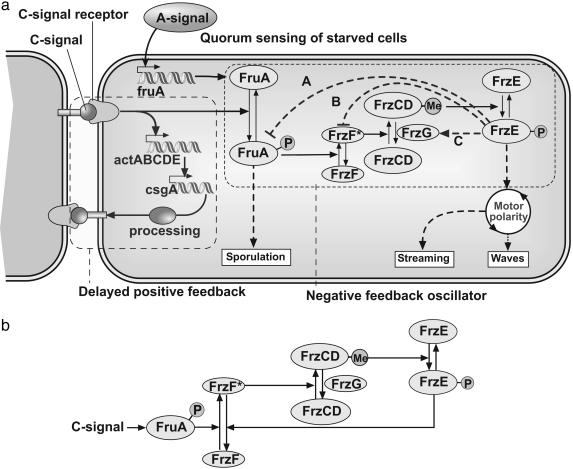
\includegraphics[width=0.7\textwidth]{images/myxococcus_diagram.jpg}
\end{center}
Translate this diagram into a system of three ODEs for the relative concentrations of Frz, FrzCD, and FrzE. Each species is regulated by saturating (Goldbeter-Koshland-type) kinetics of the form:
$$ \frac{k \cdot [\text{substrate}]}{K_m + [\text{substrate}]} $$
Include the \lstinline|external_signal| parameter as an additive modifier to $\bar{k}_0$.

\subsubsection*{Implementation part}
\textbf{Implement:} a function \lstinline|frz_pathway_rhs(state, t, external_signal)|.

\begin{center}
\renewcommand{\arraystretch}{2.0}
\begin{tabular}{r | c | c | c | c}
\toprule
\textbf{Symbol} & $[Frz, FrzCD, FrzE]$ & $t$ & $S$ & $[dFrz, dFrzCD, dFrzE]$ \\ \midrule
\textbf{Argument} & \lstinline|state| & \lstinline|t| & \lstinline|external_signal| & \lstinline|return| \\ \midrule
\textbf{Type} & \lstinline|list| & \lstinline|float| & \lstinline|float| & \lstinline|list| \\
\bottomrule
\end{tabular}
\end{center}

\textbf{Test:} Press ``L3 Myxococcus Signal'' button. View the live oscillograph.

\section*{Problem 4: Saccharomyces cerevisiae Glycolytic Oscillations}

\subsubsection*{Mathematical part}
The yeast glycolysis feedback loop (Bier-Bakker-Westerhoff model):
\begin{center}
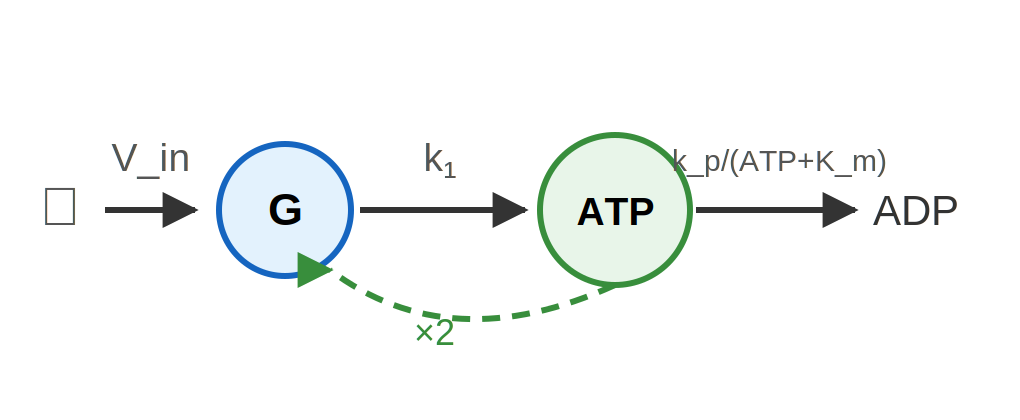
\includegraphics[width=0.55\textwidth]{images/glycolysis_bier.png}
\end{center}
The reaction network consists of three processes:
\begin{enumerate}
    \item \textbf{Glucose influx:} External glucose enters the cell at constant rate $V_{in}$.
    \item \textbf{Phosphofructokinase (PFK):} Glucose is phosphorylated by ATP with rate $k_1 \cdot G \cdot ATP$. Each glucose consumed produces \textbf{two} ATP molecules.
    \item \textbf{ATP consumption:} ATP is consumed by downstream metabolism with Michaelis-Menten kinetics: $k_p \cdot ATP / (ATP + K_m)$.
\end{enumerate}

\textbf{Task:} Write the ODEs for $G$ and $ATP$. Use parameters $V_{in} = 0.36$, $k_1 = 0.02$, $k_p = 6.0$. Analytically solve for the fixed point $(G_{eq}, ATP_{eq})$ by setting $dG/dt = 0$ and $dATP/dt = 0$.

\textbf{Hint:} The feedback arrow from ATP to the PFK reaction means that ATP is both a \emph{substrate} (consumed) and a \emph{product} (produced) of that reaction step. This autocatalytic feedback is what generates the oscillations.

\subsubsection*{Implementation part}
\textbf{Implement:} functions \lstinline|glycolysis_rhs(state, t, Km)| and \lstinline|glycolysis_fixed_point(Km)|.

\begin{center}
\renewcommand{\arraystretch}{2.0}
\begin{tabular}{r | c | c | c | c}
\toprule
\textbf{Argument} & \lstinline|state| & \lstinline|t| & \lstinline|Km| & \lstinline|return| \\ \midrule
\textbf{Type} & \lstinline|list| & \lstinline|float| & \lstinline|float| & \lstinline|list| \\
\bottomrule
\end{tabular}
\end{center}

\vspace{0.2cm}
\begin{center}
\renewcommand{\arraystretch}{2.0}
\begin{tabular}{r | c | c}
\toprule
\textbf{Argument} & \lstinline|Km| & \lstinline|return| \\ \midrule
\textbf{Type} & \lstinline|float| & \lstinline|tuple(float, float)| \\
\bottomrule
\end{tabular}
\end{center}

\textbf{Test:} Press ``L4 Glycolysis Bifurcation''. The dashboard shows a bifurcation diagram (left), phase portrait with nullclines (center), and oscillograph (right). Drag $K_m$ below the Hopf bifurcation point and observe the birth of limit-cycle oscillations.

\section*{Problem 5: Bio-switch with Mutual Activation}

\subsubsection*{Mathematical part}
The Goldbeter-Koshland zero-order ultrasensitivity mutual activation switch:
\begin{center}
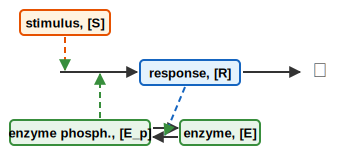
\includegraphics[width=0.55\textwidth]{images/bioswitch_gk.png}
\end{center}
The network topology features a Response $R$ and an Enzyme $E$ that mutually activate each other, forming a true bistable positive feedback loop. In the presence of a transient stimulus $S(t)$:
\begin{itemize}
    \item $R$ is produced at a basal rate proportional to the active (phosphorylated) enzyme $E_p = [E]_{tot} - [E]$, plus the stimulus $S(t)$.
    \item $R$ degrades linearly at rate $k_{R1} [R]$.
    \item $R$ acts as a kinase, phosphorylating the inactive enzyme $E \to E_p$ with Michaelis-Menten kinetics.
    \item A constitutive phosphatase dephosphorylates $E_p \to E$.
\end{itemize}

Because the Michaelis constants $K_0, K_1$ are extremely small compared to $E_{tot}$, the enzyme operates in the zero-order saturated regime. This generates the steep ultrasensitive response necessary for biochemical memory (hysteresis).

\textbf{Task:} Write the ODEs for $R$ and $E$. Use parameters: $k_{R0} = 0.22$, $k_{R1} = 0.001$, $k_{E0} = 0.8$, $k_{E1} = 0.01$, $K_0 = 0.01$, $K_1 = 0.01$, $E_{tot} = 0.5$.

\subsubsection*{Implementation part}
\textbf{Implement:} a function \lstinline|bioswitch_rhs(state, t, S)| that returns the derivatives \lstinline|[dR/dt, dE/dt]|.

\begin{center}
\renewcommand{\arraystretch}{2.0}
\begin{tabular}{r | c | c | c | c}
\toprule
\textbf{Argument} & \lstinline|state| & \lstinline|t| & \lstinline|S| & \lstinline|return| \\ \midrule
\textbf{Type} & \lstinline|list| & \lstinline|float| & \lstinline|float| & \lstinline|list| \\
\bottomrule
\end{tabular}
\end{center}

\textbf{Test:} Press ``L5 Bio-switch''. The dashboard shows an Interactive Pulse Experiment spanning 60,000 seconds. Click and drag the orange dot to change the intensity and timing of the Gaussian stimulus pulse $S(t)$. Observe how the response $[R]$ either falls back to zero or permanently flips to the high state (biochemical memory) depending on the pulse shape.

\section*{Problem 6: Cell Cycle Checkpoint (Cusp Catastrophe)}

\subsubsection*{Mathematical part}

\begin{center}
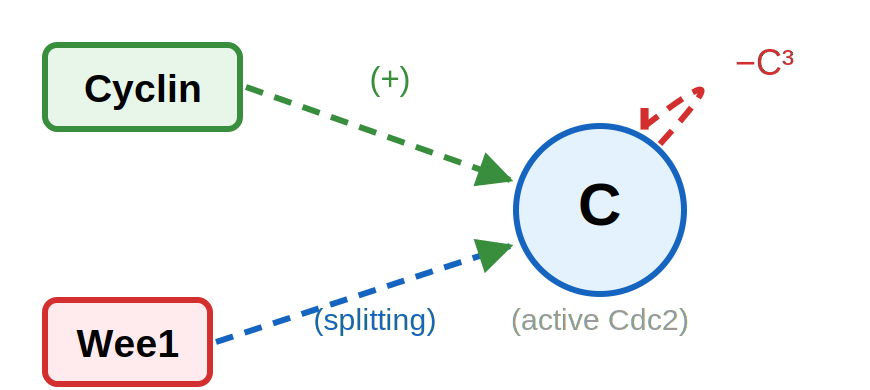
\includegraphics[width=0.45\textwidth]{images/cusp_cell_cycle.png}
\end{center}

The cell cycle checkpoint is governed by the interplay between Cyclin and Wee1 kinase. We can build a phenomenological model directly from the network scheme:
\begin{enumerate}
    \item Cyclin drives the production of active Cdc2 ($C$).
    \item Wee1 interacts with $C$ to create an autocatalytic-like splitting effect (rate proportional to $Wee1 \cdot C$).
    \item $C$ undergoes a high-order self-inhibition (cubic degradation, $-C^3$).
\end{enumerate}

Assuming all rate constants are exactly $1.0$, derive the governing differential equation for $C$.

The equilibrium manifold is a folded surface in $(Wee1, Cyclin, C)$ space. When a trajectory crosses the fold boundary, the system undergoes a \textbf{catastrophic jump} to the other stable branch.

\textbf{Task:} Find the steady-state concentration(s) of $C$. You should get a cubic polynomial, there may be up to 3 real roots (bistability). To account for \textbf{hysteresis} (biochemical memory), your function must evaluate all roots and return the real root that is \emph{closest} to the system's current state.

\subsubsection*{Implementation part}
\textbf{Implement:} a function \lstinline|cell_cycle_steady_state(cyclin, wee1, current_C)| that returns the closest stable real root.

\begin{center}
\renewcommand{\arraystretch}{2.0}
\begin{tabular}{r | c | c | c | c}
\toprule
\textbf{Argument} & \lstinline|cyclin| & \lstinline|wee1| & \lstinline|current_C| & \lstinline|return| \\ \midrule
\textbf{Type} & \lstinline|float| & \lstinline|float| & \lstinline|float| & \lstinline|float| \\
\bottomrule
\end{tabular}
\end{center}

\textbf{Test:} Press ``L6 Cusp Catastrophe''. The dashboard shows the 3D equilibrium manifold (left) and the 2D control plane (right) with the cusp-shaped bistable region highlighted. Click and drag in the control plane to explore hysteresis. When your cursor crosses the fold line, observe the catastrophic jump as your function snaps to the newly stable root.

\section*{\textcolor{red}{Submission}}
Submit the file \texttt{implementation\_tasks.py}.

\end{document}
